Considera la funció
\[
f(x)=\frac{x^2}{x^2-4} .
\]

\begin{apartats}

\apartat[1,25]{1}
Troba'n el domini, els punts de tall amb els eixos i totes les asímptotes.

\begin{solucio}
\textbf{Domini}: $x^2-4=(x-2)(x+2)\neq0$, és a dir $\mathbb{R}\setminus\{-2,2\}$. Com que
$f(-x)=f(x)$, la gràfica és simètrica respecte de l'eix $OY$.\\
\textbf{Talls}: $f(x)=0$ només si $x=0$, i $f(0)=0$: la gràfica passa per l'origen $(0,0)$.\\
\textbf{Verticals}: en $x=2$ i en $x=-2$ el numerador val $4\neq0$. En $x=2$ els laterals valen $-\infty$
(per l'esquerra) i $+\infty$ (per la dreta), i en $x=-2$, $+\infty$ i $-\infty$: asímptotes
$\boxed{x=2}$ i $\boxed{x=-2}$.\\
\textbf{Horitzontal}: mateix grau, i $\lim_{x\to\pm\infty}f(x)=1$: asímptota $\boxed{y=1}$. Per tant,
no n'hi ha cap d'obliqua.
\end{solucio}

\begin{nomesllarg}
\apartat{0,75}
Estudia'n la curvatura.

\begin{solucio}
$f'(x)=\dfrac{-8x}{\left(x^2-4\right)^2}$ i, derivant un altre cop i simplificant,
$f''(x)=\dfrac{8\left(3x^2+4\right)}{\left(x^2-4\right)^3}$.\\
El numerador és sempre positiu, i el signe és el de $\left(x^2-4\right)^3$: $f''<0$ a $(-2,2)$, on la
funció és \textbf{còncava}, i $f''>0$ a $(-\infty,-2)$ i a $(2,+\infty)$, on és \textbf{convexa}.\\
No hi ha punts d'inflexió: $f''$ no s'anul·la mai, i en $x=\pm2$ la funció no està definida.
\end{solucio}
\end{nomesllarg}

\begin{tria}{estudi-tasca}
\itemtria{original}{0,75}{1,25}
Estudia'n la monotonia i els extrems, i representa la funció.

\begin{solucio}
$f'(x)=\dfrac{2x\left(x^2-4\right)-x^2\cdot2x}{\left(x^2-4\right)^2}=\dfrac{-8x}{\left(x^2-4\right)^2}$. El
denominador és positiu, i el signe és el de $-8x$: $f$ \textbf{creix} a $(-\infty,-2)$ i a $(-2,0)$, i
\textbf{decreix} a $(0,2)$ i a $(2,+\infty)$.\\
\textbf{Màxim relatiu} $(0,0)$. No hi ha cap mínim.
\begin{center}
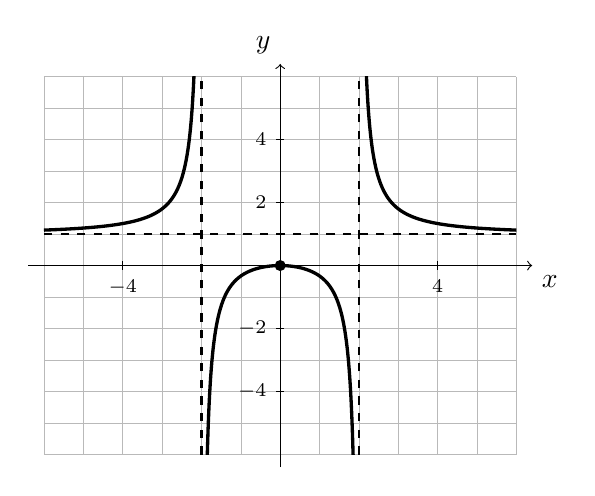
\begin{tikzpicture}[x=0.5cm,y=0.4cm]
  \draw[gray!55,very thin,step=1] (-6,-6) grid (6,6);
  \draw[->] (-6.4,0) -- (6.4,0) node[below right] {$x$};
  \draw[->] (0,-6.4) -- (0,6.4) node[above left] {$y$};
  \foreach \i in {-4,4} \draw (\i,0.15) -- (\i,-0.15) node[below,font=\scriptsize] {$\i$};
  \foreach \j in {-4,-2,2,4} \draw (0.1,\j) -- (-0.1,\j) node[left,font=\scriptsize] {$\j$};
  \draw[dashed,thick] (-2,-6) -- (-2,6);
  \draw[dashed,thick] (2,-6) -- (2,6);
  \draw[dashed,thick] (-6,1) -- (6,1);
  \begin{scope}
    \clip (-6,-6) rectangle (6,6);
    \draw[\colorgrafica,very thick,domain=-6:-2.1,samples=120,smooth] plot (\x,{(\x*\x)/(\x*\x-4)});
    \draw[\colorgrafica,very thick,domain=-1.9:1.9,samples=120,smooth] plot (\x,{(\x*\x)/(\x*\x-4)});
    \draw[\colorgrafica,very thick,domain=2.1:6,samples=120,smooth] plot (\x,{(\x*\x)/(\x*\x-4)});
  \end{scope}
  \fill (0,0) circle (2pt);
\end{tikzpicture}
\end{center}
\end{solucio}

\itemtria{posicio-asimptota}{0,75}{1,25}
Estudia'n la monotonia i els extrems. La gràfica talla mai l'asímptota horitzontal? A quina banda
en queda?

\begin{solucio}
$f'(x)=\dfrac{-8x}{\left(x^2-4\right)^2}$: $f$ \textbf{creix} a $(-\infty,-2)$ i a $(-2,0)$, i
\textbf{decreix} a $(0,2)$ i a $(2,+\infty)$. \textbf{Màxim relatiu} $(0,0)$.\\
$f(x)-1=\dfrac{x^2-\left(x^2-4\right)}{x^2-4}=\dfrac{4}{x^2-4}$, que no s'anul·la mai: la gràfica
\textbf{no talla} l'asímptota $y=1$.\\
Si $|x|>2$, $f(x)-1>0$, i la gràfica queda \textbf{per sobre} de l'asímptota; si $|x|<2$, queda
\textbf{per sota}.
\end{solucio}
\end{tria}

\end{apartats}
